%*******************************************
% Lab 04: ALU
%*******************************************
\chapter{Arithmetic Logic Unit (ALU)}\label{lab04}

\section{Purpose}

In this lab you will build an \acf{ALU}. An \ac{ALU} is an important digital logic device used to perform all sorts of arithmetic and logic functions in a circuit. The commercial 74181 \ac{ALU} has two four-bit data inputs along with a one-bit mode (M) and a four-bit select input. Depending on those settings, the device will complete one of the functions listed in Table \ref{tab0301}.

\begin{table}[H]
	\sffamily
	\newcommand{\head}[1]{\textcolor{white}{\textbf{#1}}}		
	\begin{center}
		\rowcolors{2}{gray!10}{white} % Color every other line a light gray
		\begin{tabular}{ccc} 
			\rowcolor{black!75}
			\head{Select} & \head{Logic (M=1)} &\head{Arithmetic (M=0)} \\
			0000 & A' & A \\
			0001 & (A + B)' & A + B \\
			0010 & A'B & A + B' \\
			0011 & Logical 0 & minus 1 (2's Comp) \\
			0100 & (AB)' & A + AB' \\
			0101 & B' & (A + B) plus AB' \\
			0110 & A XOR B & A minus B minus 1 \\
			0111 & AB' & AB' minus 1 \\
			1000 & A' + B & A plus AB \\
			1001 & (A XOR B)' & A plus B \\
			1010 & B & (A + B') plus AB \\
			1011 & AB & AB minus 1 \\
			1100 & Logical 1 & A plus A \\
			1101 & A + B' & (A + B) plus A \\
			1110 & A + B & (A + B') plus A \\
			1111 & A & A minus 1
		\end{tabular}
	\end{center}
	\caption{Function Table for 74181 ALU}
	\label{tab0301}
\end{table}

Notes: in the ``Arithmetic'' column, the + sign indicates logic \textit{OR} while the words \textit{plus} and \textit{minus} indicate arithmetic add and subtract operations. The value of \textit{A plus A} is the same as shifting the bits left to the next most significant position.

The \ac{ALU} built in this lab is not as complex as a 74181 \ac{IC}, however it demonstrates the basic functions of an \ac{ALU}.

\section{Procedure}

\marginpar{This is a rather complex circuit so several completed subcircuits are provided.}Load the \ac{ALU} starter circuit in \textit{Logisim-evolution}. That starter circuit already has the \lstinline[columns=fixed]|main|, \lstinline[columns=fixed]|ALU|, and \lstinline[columns=fixed]|Arithmetic| subcircuits completed.

\subsection{main}

The \lstinline[columns=fixed]|main| circuit does nothing more than provide a human-friendly interface for the rest of the \ac{ALU}. That interface include two four-bit inputs (labeled \textit{InA} and \textit{InB}), a three-bit select, a one-bit mode, a carry-in and carry-out bit (so the \ac{ALU} could be chained to another to create an eight-bit device), a \textit{compare} output (TRUE if the two inputs are equal), and a four-bit output (labeled \textit{ALUOut}). In operation, numbers are entered on \textit{InA} and \textit{InB}, the mode and select are set, and then the result is read on \textit{ALUOut}.

\begin{figure}[H]
	\centering
	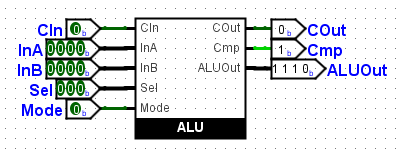
\includegraphics[width=\maxwidth{.95\linewidth}]{gfx/04-01}
	\caption{ALU main}
	\label{fig:04-01}
\end{figure}

\subsection{ALU}

The \lstinline[columns=fixed]|ALU| subcircuit contains the logic that routes \textit{InA}, \textit{InB}, and \textit{Sel} to two other subcircuits, \lstinline[columns=fixed]|Arithmetic| or \lstinline[columns=fixed]|Logic|. It then uses a multiplexer to route the output of one of those subcircuits to an output port depending on the setting of the \textit{Mode} bit. Note that the inputs are sent to both subcircuits but only the output specified by the \textit{Mode} is returned to the user. This type of logic is also used in the \lstinline[columns=fixed]|Arithmetic| circuit.

\begin{figure}[H]
	\centering
	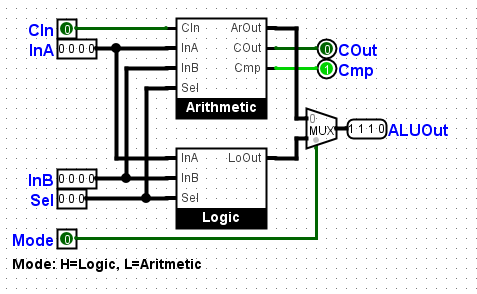
\includegraphics[width=\maxwidth{.95\linewidth}]{gfx/04-02}
	\caption{ALU Subcircuit}
	\label{fig:04-02}
\end{figure}

\subsection{Arithmetic}

This subcircuit contains numerous devices from the \textit{Arithmetic} library and they are all wired appropriately for whatever operation is selected. The concept for this subcircuit is rather simple but routing the wiring to all of the devices is challenging.

Notice that two multiplexers are necessary since the circuit provides two different outputs. The top multiplexer routes the four-bit solution and the bottom multiplexer routes the carry-out bit. The \textit{compare} output is always active since it is comparing the input signals and does not rely on the function that is selected.

\begin{figure}[H]
	\centering
	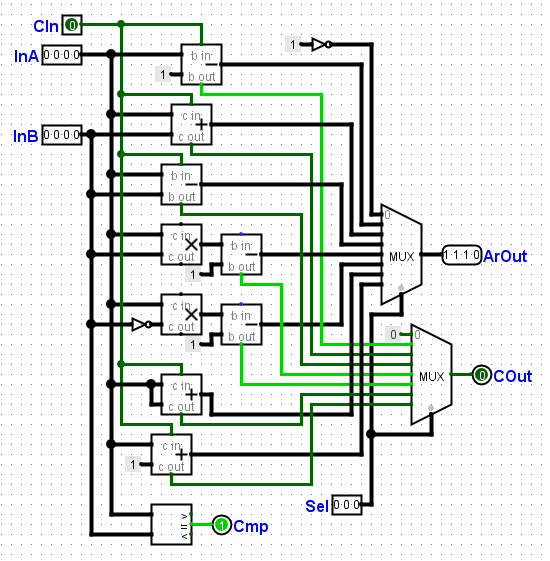
\includegraphics[width=\maxwidth{.95\linewidth}]{gfx/04-03}
	\caption{Arithmetic Subcircuit}
	\label{fig:04-03}
\end{figure}

\subsection{Challenge}

In the starter circuit, the \lstinline[columns=fixed]|Logic| subcircuit is only a shell with three inputs and one output.

\begin{figure}[H]
	\centering
	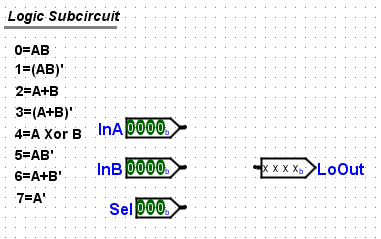
\includegraphics[width=\maxwidth{.95\linewidth}]{gfx/04-04}
	\caption{Logic Subcircuit}
	\label{fig:04-04}
\end{figure}

Complete that subcircuit by adding the necessary logic gates and wiring, similar to the \lstinline[columns=fixed]|Arithmetic| subcircuit. This subcircuit is much simpler than the \lstinline[columns=fixed]|Arithmetic| subcircuit since there are no carry-in, carry-out, or compare bits. When completed, the subcircuit only needs eight logic gates and a multiplexer added to the starter.

\subsection{Testing the Circuit}

The \lstinline[columns=fixed]|ALU| should be tested by entering several values on \textit{InA} and \textit{InB} and then select all possible arithmetic and logic operations. The outputs for each check should be accurate.

\section{Deliverable}

To receive a grade for this lab, complete the Challenge. Be sure the standard identifying information is at the top left of the \textit{main} circuit, similar to this: 

\bigskip
% The minipage environment keeps the three lines together - no page break.
\begin{minipage}{\linewidth}
	\begin{verbatim}
	George Self
	Lab 04: ALU
	February 18, 2018
	\end{verbatim}
\end{minipage}
\bigskip

Save the file with this name: \emph{\texttt{Lab04\_ALU}} and submit that file for grading.
